% NERACA: a plain guide to the app -- features, how it works, data, and method
% Compile: pdflatex main.tex (twice)
\documentclass[11pt,a4paper]{article}
\usepackage[T1]{fontenc}
\usepackage[utf8]{inputenc}
\usepackage[sc]{mathpazo}
\usepackage[scaled=0.92]{helvet}
\renewcommand{\ttdefault}{lmtt}
\usepackage{microtype}
\usepackage[a4paper,left=24mm,right=24mm,top=25mm,bottom=25mm]{geometry}
\usepackage{amsmath,amssymb}
\usepackage[table]{xcolor}
\usepackage{booktabs,tabularx,array}
\usepackage{xltabular}
\usepackage{needspace}
\usepackage{enumitem}
\usepackage{titlesec}
\usepackage{fancyhdr}
\usepackage[most]{tcolorbox}
\usepackage{tikz}
\usetikzlibrary{arrows.meta,positioning,calc}
\usepackage{caption}
\usepackage{float}
\usepackage[hidelinks]{hyperref}
\usepackage{xurl}

% ---------- colours (same palette as the NERACA research report) ----------
\definecolor{ink}{HTML}{10232B}
\definecolor{muted}{HTML}{52514E}
\definecolor{accent}{HTML}{1C5CAB}
\definecolor{accentsoft}{HTML}{E6EFFA}
\definecolor{warm}{HTML}{B4491E}
\definecolor{warmsoft}{HTML}{FCEDE6}
\definecolor{green}{HTML}{0F7A55}
\definecolor{greensoft}{HTML}{E4F4EE}
\definecolor{line}{HTML}{C9D3D8}
\color{ink}
\hypersetup{colorlinks=true,linkcolor=accent,urlcolor=accent}

% ---------- headings and spacing ----------
\titleformat{\section}{\sffamily\bfseries\Large\color{ink}}{\thesection}{0.7em}{}
\titleformat{\subsection}{\sffamily\bfseries\large\color{ink}}{\thesubsection}{0.6em}{}
\titleformat{\subsubsection}{\sffamily\bfseries\normalsize\color{accent}}{}{0em}{}
\titlespacing*{\section}{0pt}{16pt}{6pt}
\titlespacing*{\subsection}{0pt}{12pt}{4pt}
\titlespacing*{\subsubsection}{0pt}{9pt}{2pt}
\setlength{\parindent}{0pt}
\setlength{\parskip}{6pt}
\setlist{itemsep=2pt,topsep=3pt,leftmargin=1.5em}
\renewcommand{\arraystretch}{1.25}
\captionsetup{font={small,sf},labelfont=bf,skip=6pt}

\setlength{\headheight}{14pt}
\pagestyle{fancy}
\fancyhf{}
\fancyhead[L]{\small\sffamily\color{muted}NERACA: a plain guide to the app}
\fancyhead[R]{\small\sffamily\color{muted}\nouppercase{\leftmark}}
\fancyfoot[C]{\small\sffamily\color{muted}\thepage}
\renewcommand{\headrulewidth}{0.3pt}
\renewcommand{\headrule}{\color{line}\hrule width\headwidth height\headrulewidth}

% ---------- boxes ----------
\newtcolorbox{inshort}{enhanced,breakable,colback=accentsoft,colframe=accentsoft,boxrule=0pt,arc=2pt,
  left=10pt,right=10pt,top=7pt,bottom=7pt,borderline west={3pt}{0pt}{accent},
  before upper={\textsf{\textbf{\color{accent}In short.}}\ }}
\newtcolorbox{plain}{enhanced,breakable,colback=greensoft,colframe=greensoft,boxrule=0pt,arc=2pt,
  left=10pt,right=10pt,top=7pt,bottom=7pt,borderline west={3pt}{0pt}{green},
  before upper={\textsf{\textbf{\color{green}In plain words.}}\ }}
\newtcolorbox{caution}{enhanced,breakable,colback=warmsoft,colframe=warmsoft,boxrule=0pt,arc=2pt,
  left=10pt,right=10pt,top=7pt,bottom=7pt,borderline west={3pt}{0pt}{warm},
  before upper={\textsf{\textbf{\color{warm}Honest limit.}}\ }}
\newtcolorbox{tryit}{enhanced,breakable,colback=white,colframe=line,boxrule=0.5pt,arc=2pt,
  left=10pt,right=10pt,top=6pt,bottom=6pt,
  before upper={\textsf{\textbf{\color{accent}On screen.}}\ }}

% ---------- provenance labels: what backs a number ----------
\definecolor{tested}{HTML}{0B6E79}
\definecolor{calc}{HTML}{6B6A66}
\definecolor{weak}{HTML}{9A7413}
\definecolor{miss}{HTML}{A61B29}
\definecolor{scen}{HTML}{6B3FA0}
\newcommand{\pv}[2]{{\setlength{\fboxsep}{1.3pt}\colorbox{#1}{\textcolor{white}{\sffamily\bfseries\fontsize{6.3}{7}\selectfont #2}}}}
\newcommand{\Off}{\pv{accent}{OFFICIAL}}
\newcommand{\Mea}{\pv{green}{MEASURED}}
\newcommand{\Tst}{\pv{tested}{TESTED}}
\newcommand{\Calc}{\pv{calc}{CALCULATED}}
\newcommand{\Wk}{\pv{weak}{WEAK}}
\newcommand{\Scn}{\pv{scen}{SCENARIO}}
\newcommand{\Mis}{\pv{miss}{MISSING}}
\newcommand{\Pass}{\pv{green}{PASS}}
\newcommand{\Fail}{\pv{warm}{FAIL}}
\newcommand{\Wait}{\pv{calc}{WAITING}}

% ---------- small helpers ----------
\newcommand{\Mm}{\,Mm$^{3}$}
\newcommand{\Mmyr}{\,Mm$^{3}$/yr}
\newcommand{\mthree}{m$^{3}$}
\newcommand{\route}[1]{\texttt{\small #1}}
\newcolumntype{L}[1]{>{\raggedright\arraybackslash}p{#1}}
\newcolumntype{Y}{>{\raggedright\arraybackslash}X}
\tikzset{
  box/.style={draw=line,fill=white,rounded corners=2pt,align=center,font=\sffamily\small,inner sep=5pt,text=ink},
  boxa/.style={box,draw=accent,fill=accentsoft},
  boxg/.style={box,draw=green,fill=greensoft},
  boxw/.style={box,draw=warm,fill=warmsoft},
  arr/.style={-{Stealth[length=5pt]},draw=muted,line width=0.6pt},
  lab/.style={font=\sffamily\scriptsize,text=muted}
}

\begin{document}

% =====================================================================================
\thispagestyle{empty}
\begin{center}
{\sffamily\scriptsize\color{muted} ASEAN Geospatial Challenge 2027 \textbullet\ National Level: Indonesia \textbullet\ 20 November 2026}\\[4mm]
{\sffamily\bfseries\fontsize{26}{30}\selectfont\color{ink} NERACA}\\[2mm]
{\sffamily\Large\color{accent} A plain guide to the app}\\[1.5mm]
{\sffamily\normalsize\color{muted} What it does, how it works, where the numbers come from, and how they are made}
\end{center}
\vspace{2mm}

\begin{tcolorbox}[enhanced,colback=accent,colframe=accent,boxrule=0pt,arc=2pt,left=10pt,right=10pt,top=8pt,bottom=8pt]
\sffamily\color{white}\textbf{The app in one paragraph.} Semarang, on the north coast of Central Java, is sinking
by up to about 9--11\,cm a year, mostly because groundwater is pumped out faster than it refills. NERACA
(Indonesian for ``balance sheet'') is a map-based web app that keeps a groundwater \emph{account book} for
the province. It answers three questions: \textbf{(A)} how much groundwater is used compared with how much
is declared, and what the difference is worth in tax; \textbf{(B)} which new large buildings an inspector
should visit first; and \textbf{(C)} where piped water should replace pumps, and whether it already slowed
the sinking. Every number on screen carries a small label that says what backs it.
\end{tcolorbox}

\vspace{1mm}
\textbf{Who this guide is for.} Anyone who wants to understand the app without reading the research
report: judges, team members, officials, or a new developer. It is written in plain words. Where a formula
helps, it is shown once and then explained in a sentence. The full research reasoning lives in the
companion report, \emph{NERACA: Groundwater Accounts} (\texttt{docs/groundwater-accounts-latex}).

\setcounter{tocdepth}{2}
{\small\tableofcontents}

% =====================================================================================
\section{What NERACA is}\label{sec:what}

\subsection{The problem in three facts}

\begin{enumerate}
\item \textbf{The city is sinking.} Satellite radar shows the fastest parts of Semarang sinking about
  113\,mm a year in 2014--2017 and still about 89\,mm a year in 2023--2026 \Mea.
\item \textbf{Declared pumping is falling on paper.} Registered groundwater use in Kota Semarang was
  27.7\Mm\ in 2018 and 10.1\Mm\ in 2023 \Off. Nobody knows how much of that fall is real and how much is
  under-reporting or wells that were never registered.
\item \textbf{Industry runs on its own wells.} The city water company (PDAM) sold only 0.22\Mm\ of piped
  water to all of Semarang's industry in 2022 \Off. Most of the city is a zone where new wells are banned.
\end{enumerate}

\subsection{Three questions, three modules}

\begin{center}
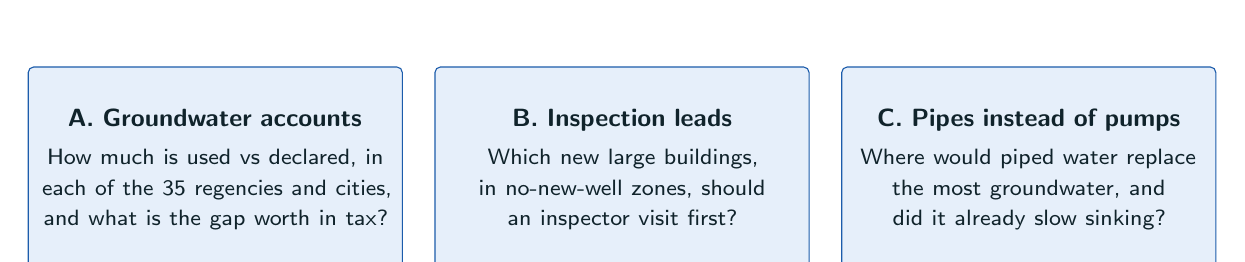
\begin{tikzpicture}[node distance=4mm]
\node[boxa,text width=44mm,minimum height=26mm] (a) {\textbf{A. Groundwater accounts}\\[3pt]
  \footnotesize How much is used vs declared, in each of the 35 regencies and cities, and what is the gap
  worth in tax?};
\node[boxa,text width=44mm,minimum height=26mm,right=of a] (b) {\textbf{B. Inspection leads}\\[3pt]
  \footnotesize Which new large buildings, in no-new-well zones, should an inspector visit first?};
\node[boxa,text width=44mm,minimum height=26mm,right=of b] (c) {\textbf{C. Pipes instead of pumps}\\[3pt]
  \footnotesize Where would piped water replace the most groundwater, and did it already slow sinking?};
\end{tikzpicture}
\end{center}

\subsection{What the app is \emph{not}}

\begin{itemize}
\item \textbf{It is not a well detector.} Our earlier research tested whether satellites can point at
  single wells. They cannot: registered deep wells do not sit on faster-sinking ground, and the sinking
  pattern mostly follows how thick the soft clay is. So the app never draws a well from a sinking map.
\item \textbf{It is not a tax bill.} It shows ranges and scenarios. It never prints a single
  ``lost revenue'' headline that the data cannot support.
\item \textbf{It does not hide failures.} Each method has a check with a pass mark written down before the
  check ran. Five checks have run and failed so far; the app shows them (Section~\ref{sec:checks}).
\end{itemize}

\subsection{Who uses it}

There is no login. On the sign-in screen you pick a role, and the app shows the views that role needs.
This is a demo gate, not security.

\begin{center}
\small
\begin{tabularx}{\linewidth}{@{}L{24mm}Y@{}}
\toprule
\textbf{Role} & \textbf{What they see and do}\\
\midrule
Public & The accounts map, the checks and the source list. Leads are shown only as counts per district,
  never as addresses.\\
Regulator & Accounts, the official price table, the billing check, validation and sources.\\
Inspector & The full lead list and lead cards with satellite images, and a form to record each field
  visit.\\
Planner & Accounts, the pipe-priority map with its weight sliders, the sinking periods and the SPAM
  Semarang Barat test.\\
\bottomrule
\end{tabularx}
\end{center}

% =====================================================================================
\section{How to read any number}\label{sec:labels}

\begin{inshort}
Every number in the app has a coloured label next to it. The label tells you \emph{what kind of evidence}
backs the number. Click it to see the source.
\end{inshort}

\begin{center}
\small
\begin{tabularx}{\linewidth}{@{}l Y L{50mm}@{}}
\toprule
\textbf{Label} & \textbf{Means} & \textbf{Example}\\
\midrule
\Off & Taken from a government regulation or official open data, as published. & Declared use, the
  price table\\
\Mea & Measured by a satellite or in the field. & Sinking rates, new-roof size\\
\Tst & Made by our own method, and the method passed a test fixed in advance. & The Kota Semarang use
  estimate\\
\Calc & Plain arithmetic on backed inputs; usually a range. & The gap, tax per \mthree\\
\Wk & Comes from one secondary source only (news, one database); to be confirmed. & Some building
  classes, the 20\,\% tax rate\\
\Scn & An assumption that \emph{you} set, for example with a slider. & ``What if 5\Mm\ is undeclared?''\\
\Mis & Not obtained yet. The app says so and never draws it as zero. & PDAM pipe network map\\
\bottomrule
\end{tabularx}
\end{center}

Three habits follow from this:
\begin{itemize}
\item \textbf{Ranges, not single numbers.} When something is uncertain, the app shows low, middle and high
  values (often written P10 / P50 / P90: a 1-in-10 low case, the middle case, and a 1-in-10 high case).
\item \textbf{Missing is shown as missing.} An empty layer comes with a reason, not with zeros or an
  invented shape.
\item \textbf{Every source has an entry.} The source register lists 49 sources, each with publisher,
  link and label. It is on the Methods screen.
\end{itemize}

% =====================================================================================
\section{A tour of the app}\label{sec:tour}

The app is a desktop web app built around one map. A top bar switches between the three modules and the
Methods page; a dropdown switches the role.

\begin{center}
\small
\begin{tabularx}{\linewidth}{@{}L{34mm}L{35mm}Y@{}}
\toprule
\textbf{Address} & \textbf{Screen} & \textbf{What you can do there}\\
\midrule
\route{/} & Landing page & Read what the app is and enter it.\\
\route{/sign-in} & Role picker & Choose public, regulator, inspector or planner.\\
\route{/accounts} & Accounts, Central Java & See all 35 regencies and cities on a map; pick a year and a
  measure; open one region.\\
\route{/accounts/[id]} & Account detail & Declared vs estimated use, the gap, the price, the scenario slider,
  the billing check and the history.\\
\route{/accounts/asean} & ASEAN comparison & See which data exist for Central Java, Jakarta, Ho Chi Minh
  City, Bangkok and Manila.\\
\route{/leads} & Inspection leads & The lead map, the four-filter funnel, and the map layers (zones, piped
  coverage, wells).\\
\route{/leads/[id]} & Lead detail & Before/after satellite images, why it is a lead, and the field-visit
  form.\\
\route{/leads/validation} & Hit rate and checks & Field results per building class and the Arizona test.\\
\route{/pipes} & Pipe priority & The 4\,km priority map, its weight sliders and the sinking periods.\\
\route{/pipes/spam} & SPAM Semarang Barat & The before/after test of the new water supply.\\
\route{/methods} & Methods and evidence & How each layer is made, all checks, all sources.\\
\bottomrule
\end{tabularx}
\end{center}

\subsection{Module A: groundwater accounts}

\begin{tryit}
A map of Central Java's 35 regencies and cities (\emph{kabupaten/kota}). Pick a year (2020--2023) and what
the colours show: \emph{tax gap}, \emph{declared volume}, \emph{estimated use}, or \emph{declared $\div$
estimated} (how much of the use is reported). Click a region to open its account.
\end{tryit}

The account page for one region shows:
\begin{itemize}
\item \textbf{Declared use} from the provincial energy and mines office (ESDM) \Off, and its history
  2020--2023.
\item \textbf{Estimated use} as a range, \Tst\ for Kota Semarang and \Calc\ (marked ``model'') elsewhere.
\item \textbf{The gap} between them, as a range that can go below zero.
\item \textbf{The price}: the official groundwater price per \mthree\ and the tax on it, with the full
  25-row price table for the region's price zone.
\item \textbf{A scenario slider}: ``suppose this much business use is undeclared''. The app prices
  whatever you set, labelled \Scn.
\item \textbf{The billing check (V1)}: does the tax actually collected match the declared volume?
\item For Kota Semarang, extra context: the registered-use series since 1990, what PDAM sells to whom, and
  three possible reasons why declared use fell (real decline, under-reporting, unregistered wells).
\end{itemize}

The \textbf{ASEAN} screen puts Central Java next to Jakarta, Ho Chi Minh City, Bangkok and Manila. It lists,
for each, what sinking data, declared-use data, piped-water data and policy exist today, so it is clear
where an account could open next. Bangkok is shown as the success story (groundwater charge plus piped
water plus a pumping ban where pipes exist); Ho Chi Minh City cut pumping from 716,581 to 252,528\,\mthree\
a day by the end of 2024.

\subsection{Module B: inspection leads}

\begin{tryit}
A map of the Semarang--Demak area with switchable layers: the official 2022 groundwater conservation
zones (safe, vulnerable, critical, damaged, recharge), piped-water coverage per sub-district, the 467
drilled wells marked on the 2022 zone map, and the leads themselves (inspector only). A funnel shows how
many buildings survive each filter.
\end{tryit}

A \textbf{lead} is a new, large, water-using building, in a zone where new wells are banned, in a place
that piped water does not reach well. It is a suggestion to visit, not an accusation.

Opening a lead shows:
\begin{itemize}
\item Sentinel-2 satellite images of the spot \textbf{before (2022) and after (2026)};
\item its size, the year it appeared, its use class (factory, hotel, mall, hospital) and where that
  class came from;
\item the zone it sits in, the local piped-water coverage, and the sinking rate there;
\item a \textbf{field-visit form}: the inspector records what they found -- \emph{unregistered well},
  \emph{registered well}, \emph{PDAM customer} or \emph{no well} -- with a date and a note.
\end{itemize}

The \textbf{hit-rate} screen counts these visits per building class, so over time the team learns which
kinds of leads are worth the trip. The public role never sees addresses, only the number of leads per
district.

\subsection{Module C: pipes instead of pumps}

\begin{tryit}
A grid of 22 blocks, each 4\,km by 4\,km, over Semarang. Colour them by \emph{priority score}, unserved
demand, clay thickness, sinking rate or new supply. Three sliders set how much each factor counts; the
ranking updates at once. A period picker switches the sinking maps between 2014--17, 2018--22 and
2023--26.
\end{tryit}

The \textbf{SPAM Semarang Barat} screen is about one real project: a new piped-water system from the
Jatibarang reservoir that started supplying western Semarang in 2021--2024. The screen shows its capacity,
uptake and connections, and the result of a before/after test asking whether the sinking slowed more where
it arrived (Section~\ref{sec:c}, ``Did the pipes slow the sinking?'').

\subsection{Methods and evidence}

One page that explains, for every layer, what it is built from and whether it was checked: the label
legend, the path from radar and records to the three modules, the eight checks (V1--V8) with their
status, and the full source register grouped into ``radar and ground'', ``records and law'' and
``buildings and water''.

% =====================================================================================
\section{How it works under the hood}\label{sec:how}

\begin{inshort}
All the heavy work -- satellite processing, map digitising, model fitting -- is done offline by Python
scripts. They write plain data files. The server only reads those files and answers the web app. The one
thing the server writes is the inspectors' field visits.
\end{inshort}

\begin{figure}[H]
\centering
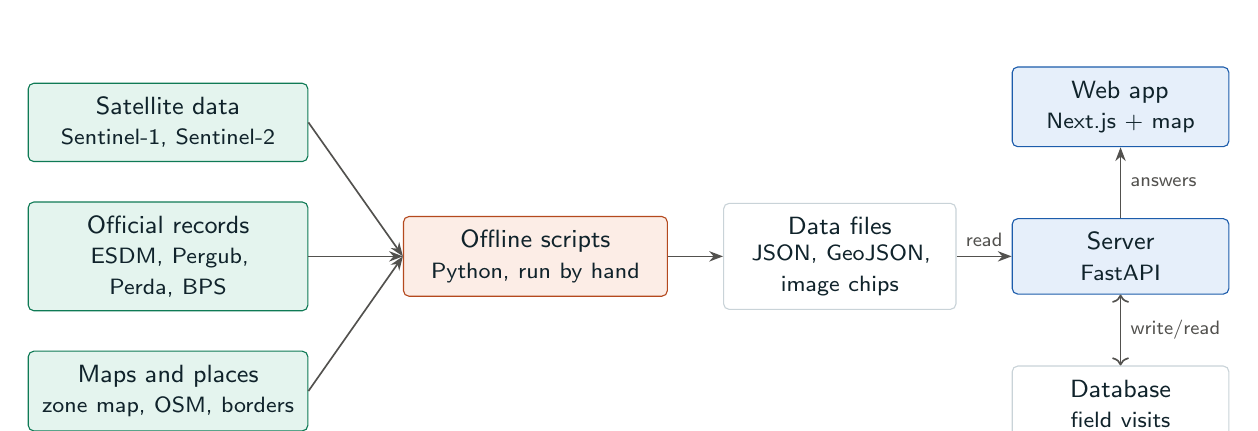
\begin{tikzpicture}[node distance=5mm and 7mm]
\node[boxg,text width=32mm] (sat) {Satellite data\\\footnotesize Sentinel-1, Sentinel-2};
\node[boxg,text width=32mm,below=of sat] (rec) {Official records\\\footnotesize ESDM, Pergub, Perda, BPS};
\node[boxg,text width=32mm,below=of rec] (map) {Maps and places\\\footnotesize zone map, OSM, borders};
\node[boxw,text width=30mm,right=12mm of rec] (scr) {Offline scripts\\\footnotesize Python, run by hand};
\node[box,text width=26mm,right=of scr] (dat) {Data files\\\footnotesize JSON, GeoJSON,\\image chips};
\node[boxa,text width=24mm,right=of dat] (api) {Server\\\footnotesize FastAPI};
\node[boxa,text width=24mm,above=9mm of api] (web) {Web app\\\footnotesize Next.js + map};
\node[box,text width=24mm,below=9mm of api] (db) {Database\\\footnotesize field visits};
\draw[arr] (sat.east) -- (scr.west);
\draw[arr] (rec.east) -- (scr.west);
\draw[arr] (map.east) -- (scr.west);
\draw[arr] (scr) -- (dat);
\draw[arr] (dat) -- node[lab,above]{read} (api);
\draw[arr] (api.north) -- node[lab,right]{answers} (web.south);
\draw[arr,<->] (api.south) -- node[lab,right]{write/read} (db.north);
\end{tikzpicture}
\caption{The data path. Everything left of ``Data files'' happens before the app runs.}
\end{figure}

\subsection{The pieces}

\begin{description}[leftmargin=0pt,labelsep=0.5em]
\item[Offline scripts.] One script per job, for example: read the ESDM open-data API, digitise the 2022 zone
  map, build the satellite composites, find new buildings, build the 4\,km grid, run the checks. Each one
  writes a file in \texttt{apps/backend/data/}. Raw downloads are kept, so the files can be rebuilt.
\item[Data files.] About fifteen small files: regions and boundaries, declared use, estimates, the price
  table, leads, pipe cells, zones, piped coverage, sources and check results. They are the app's single
  source of truth.
\item[Server.] A Python FastAPI service. It loads the data files, applies the business rules (the price
  formula, the gap, the priority ranking, the lead filters by stage) and returns JSON. Every number it
  returns carries its unit, its label and its source ids.
\item[Database.] PostgreSQL, used for one table: field visits. This is the only thing users create.
\item[Web app.] A Next.js app with MapLibre maps. It calls the server, draws the maps and charts, and shows
  the label on every value. When the server says a layer is missing, the app shows an empty state with the
  reason.
\end{description}

\subsection{Why it is built this way}

\begin{itemize}
\item \textbf{Fast and cheap to run.} Processing years of radar takes hours; reading a JSON file takes
  milliseconds. Users never wait for satellite processing.
\item \textbf{Easy to check.} Each number traces back through a file to a script and a source. Rebuilding
  gives the same file.
\item \textbf{Hard to fake.} The server cannot make up a number: if a file has no value, the answer is
  \Mis\ with a reason.
\end{itemize}

% =====================================================================================
\section{Where the data comes from, and what it is used for}\label{sec:data}

\begin{inshort}
All data are real and public. No synthetic or random numbers are used anywhere in the app.
\end{inshort}

{\small
\begin{xltabular}{\linewidth}{@{}L{38mm}L{36mm}Y l@{}}
\toprule
\textbf{Data} & \textbf{From} & \textbf{Used for} & \textbf{Label}\\
\midrule
\endhead
\multicolumn{4}{@{}l}{\textsf{\textbf{\color{accent}Satellites}}}\\
Sentinel-1 radar time series, 2014--2026 & ESA Copernicus, via COMET LiCSAR (two viewing directions) &
  Sinking rate maps and their change over time (module C); the volume estimate & \Mea\\
Sentinel-1 radar, 2022 and 2026 & ESA Copernicus, via Microsoft Planetary Computer & Checking that a new
  roof is a real building, not bare fill (module B) & \Mea\\
Sentinel-2 optical images, dry seasons 2021--2026 & ESA Copernicus, via Microsoft Planetary Computer &
  Finding new roofs and showing before/after images (module B) & \Mea\\
\addlinespace
\multicolumn{4}{@{}l}{\textsf{\textbf{\color{accent}Government records and rules}}}\\
Declared groundwater use and its value, 2020--2023 & ESDM Jawa Tengah open-data portal (CKAN API) &
  The ``declared'' side of every account, all 35 regions & \Off\\
Groundwater price formula and table & Pergub Jateng 7/2025 & Pricing the gap and the scenario & \Off\\
Earlier price tables & Pergub Jateng 19/2017 and 54/2018 & The billing check for years before 2025 &
  \Off\\
Realised groundwater tax, 2022--2024 & Perda Kota Semarang 2/2024, Kepgub Jateng 211/2025 & The billing
  check (V1) & \Off\\
PDAM sales and registered use history & Perda Kota Semarang 4/2024 & Context for Semarang; why factories
  skip filter 4 & \Off\\
2022 groundwater conservation-zone map & Dinas ESDM Jateng (vector PDF, made under Permen ESDM 31/2018)
  & Lead filter 3 (critical and damaged zones); the 467 drilled-well markers & \Off\\
Tax rate (20\,\% of the price) & Perda Kota Semarang 10/2023, via secondary sources & Tax per \mthree &
  \Wk\\
SPAM Semarang Barat facts & Cabinet Secretariat, Coordinating Ministry, news & Capacity, uptake,
  connections, service districts (module C) & \Off\,/\,\Wk\\
\addlinespace
\multicolumn{4}{@{}l}{\textsf{\textbf{\color{accent}Statistics}}}\\
Population per regency, 2020--2023 & BPS Jawa Tengah & Household well use in the regency model & \Off\\
Households by drinking-water source & BPS Jawa Tengah (Susenas) & Share of households on wells & \Off\\
Piped-water customers per sub-district & BPS Kota Semarang Dalam Angka 2024; Portal Data Demak 2025 &
  Lead filter 4 (piped coverage proxy) & \Off\\
\addlinespace
\multicolumn{4}{@{}l}{\textsf{\textbf{\color{accent}Maps, buildings and places}}}\\
Regency and city boundaries & geoBoundaries (ADM2) & The 35-region accounts map & \Off\\
Sub-district boundaries & GADM & Lead districts, coverage map, SPAM service area & \Off\\
Building footprints & Microsoft Global ML Building Footprints & Training the roof detector & \Mea\\
Annual land cover, 2017--2023 & Impact Observatory (10\,m) & Training the roof detector; the Arizona
  test & \Mea\\
Building tags, industrial land & OpenStreetMap & Lead use class; industrial land in the regency model &
  \Wk\\
Places (businesses) & Overture Maps & Lead use class where OpenStreetMap has none & \Wk\\
Soft-clay thickness & Borehole data (from the research) & Damage potential in the pipe-priority map &
  \Mea\\
\addlinespace
\multicolumn{4}{@{}l}{\textsf{\textbf{\color{accent}Reference cases (used only for checking)}}}\\
Well registry, water-provider areas, metered pumping & Arizona Department of Water Resources & Checks V4
  and V8: places where the truth is known & \Off\\
\bottomrule
\end{xltabular}}

\textbf{Our own earlier research} also feeds the app: the validated volume split, the finding that clay
explains about 80\,\% of the sinking pattern, the sinking periods, and the 4\,km demand model. Each of these
is a source in the register with its own label (\Tst\ when it passed a test, \Calc\ when it did not).

% =====================================================================================
\section{The method, step by step}\label{sec:method}

\subsection{Module A: groundwater accounts}

\begin{plain}
For each region: take what was declared, estimate what is really used, subtract, and price the difference
with the official tariff. Show every step as a range.
\end{plain}

\subsubsection{Step 1. Declared use}
Read the declared volume and its official value for each region and year (2020--2023) from the ESDM
open-data API. These are used exactly as published \Off.

\subsubsection{Step 2. Estimated use}
Two different methods, depending on the region:

\begin{itemize}
\item \textbf{Kota Semarang: the validated split} \Tst. Published studies give a total pumping figure for
  the Semarang region. Our method spreads that total over a grid of 16\,km cells, using water demand and
  the sinking map to decide how much goes where. Before trusting it, we fixed a pass mark (``within
  1.5$\times$ of the truth'') and tested it on two regions it had never seen. It passed. For the
  west--central Semarang cell it gives \textbf{27.9 / 43.8 / 54.7\Mmyr} (low / middle / high).
\item \textbf{The other 34 regions: the regency model} \Calc, \emph{not validated}. It adds two parts:
  \[
  \text{use} = \underbrace{\text{people}\times 80\text{--}150\ \text{L/day}\times\text{share on wells}}_{\text{household wells}}
  + \underbrace{\text{industrial land}\times\text{Semarang's rate}}_{\text{business wells}}
  \]
  The share on wells comes from BPS household surveys (low: households that drink well water; high: also
  those that drink bottled water, since their washing water is not asked). Industrial land comes from
  OpenStreetMap, priced at Kota Semarang's registered industrial use per hectare. Business use is never
  set below what was declared, because declared use is a floor.
\end{itemize}

\begin{caution}
The regency model is a rough guide. Run on Kota Semarang, it gives 24.6--102.7\Mm, wider than the validated
27.9--54.7. Moving pumping models between places has been wrong by 5--27$\times$ in our earlier tests.
Industry that uses river, sea or piped water makes it too high; patchy OpenStreetMap mapping makes it too
low. The app marks these estimates as ``model''.
\end{caution}

\subsubsection{Step 3. The gap}
Only business use is taxed; basic household use is exempt. So the gap removes the exempt parts first:
\[
\text{gap} = \text{estimated use} - \text{household wells} - \text{public-supply wells} - \text{declared}.
\]
Each term is a range, so the gap is a range. In the regency model the household term cancels out, and the
gap is simply \emph{business wells $-$ declared}.

\subsubsection{Step 4. The price}
The official groundwater price (NPA) comes from Pergub Jateng 7/2025:
\[
\text{NPA} = \text{HAB}\times(0.6\,S + 0.4\,P)
\]
\begin{itemize}
\item \textbf{HAB} is the base price of water in the region's price zone: Rp 2,561 (zone A), 2,795 (B) or
  2,824 (C) per \mthree.
\item \textbf{S} rates the resource: better water and no alternative source make it more valuable.
\item \textbf{P} rates the use: five use groups (from ``water sold as a product'' to ``social and public
  supply'') and five volume tiers (from 0--50 to over 2,500\,\mthree).
\end{itemize}
The server computes the whole 25-row table from this formula rather than copying it by hand; two printed
values were used to confirm it. The tax is 20\,\% of the NPA.

\begin{center}
\small
\begin{tabular}{@{}lrr@{}}
\toprule
\textbf{Use group (zone C, top volume tier)} & \textbf{NPA, Rp/\mthree} & \textbf{Tax, Rp/\mthree}\\
\midrule
K1 water sold as a product & 78,575 & 15,715\\
K2 high-risk business & 67,143 & 13,429\\
K3 medium-risk business & 55,701 & 11,140\\
K4 low-risk business & 44,269 & 8,854\\
K5 social, government, public supply & 32,826 & 6,565\\
\bottomrule
\end{tabular}
\end{center}

So in Semarang, each 1\Mm\ of undeclared business pumping is worth \textbf{Rp 8.9--13.4 billion a year} in
tax (groups K4 to K2).

\subsubsection{Step 5. The scenario slider}
Because the real undeclared volume is not known, the app does not claim one. Instead the user sets a
volume with a slider (starting at zero) and the app prices it \Scn. For example, 5\Mm\ in Semarang gives
Rp 44.3--67.1 billion a year.

\subsubsection{Step 6. The billing check (V1)}
This check needs no satellite at all. Divide the tax actually collected by the declared volume. If the
result per \mthree\ is \emph{below} the official band, money is leaking at the billing stage.

\subsubsection{Worked example: Kota Semarang, 2023}

\begin{center}
\small
\begin{tabularx}{\linewidth}{@{}L{52mm}Y l@{}}
\toprule
\textbf{Item} & \textbf{Value} & \textbf{Label}\\
\midrule
Declared use & 10,069,814\,\mthree/yr & \Off\\
Estimated use & 27.9 / 43.8 / 54.7\Mmyr & \Tst\\
Household wells (exempt) & 0--25\Mmyr & \Calc\\
Public-supply wells & 0--10\Mmyr & \Wk\\
\textbf{Gap} & \textbf{$-$17.2 to $+$44.6\Mmyr} (middle 16.2) & \Calc\\
Tax per undeclared \mthree & Rp 8,854--13,429 & \Calc\\
Declared use, priced (size of the tax base) & Rp 112--135 billion/yr & \Calc\\
Billing check V1 (2022, 2023) & Rp 2,188 and 2,245 per declared \mthree, inside the band Rp 2,100--2,480
  & \Pass\\
\bottomrule
\end{tabularx}
\end{center}

\begin{caution}
The gap runs from below zero to about 45\Mm. With today's data we cannot say there \emph{is} a gap: the
biggest unknown is how much households pump. The billing check passed, so billing matches what was
declared; any gap would be in volume that was never declared.
\end{caution}

% -------------------------------------------------------------------------------------
\subsection{Module B: inspection leads}

\begin{plain}
Find buildings that are new since the 2022 zone map, big, likely to use a lot of water, inside a zone where
new wells are banned, and not well served by piped water. List them for a visit. No scores: a building
either passes each filter or it does not.
\end{plain}

\begin{figure}[H]
\centering
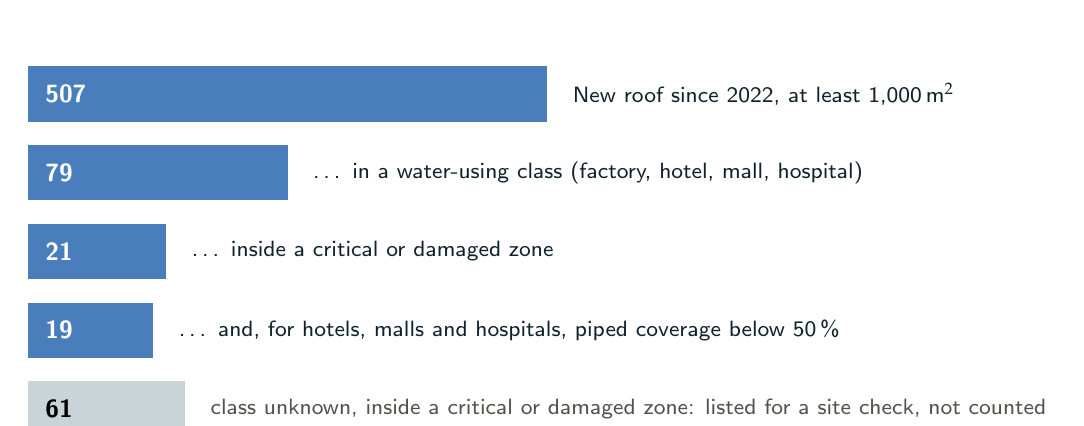
\begin{tikzpicture}[x=1mm,y=1mm,font=\sffamily\small]
\def\barh{7}
\foreach \w/\n/\t/\y in {120/507/{New roof since 2022, at least 1,000\,m$^2$}/0,
                          60/79/{\ldots\ in a water-using class (factory, hotel, mall, hospital)}/-10,
                          32/21/{\ldots\ inside a critical or damaged zone}/-20,
                          29/19/{\ldots\ and, for hotels, malls and hospitals, piped coverage below 50\,\%}/-30} {
  \fill[accent!80] (0,\y) rectangle (\w*0.55,\y+\barh);
  \node[anchor=west,text=white,font=\sffamily\bfseries\small] at (1,\y+\barh/2) {\n};
  \node[anchor=west,text=ink,font=\sffamily\footnotesize] at (\w*0.55+2,\y+\barh/2) {\t};
}
\fill[line] (0,-40) rectangle (20,-33);
\node[anchor=west,font=\sffamily\bfseries\small] at (1,-36.5) {61};
\node[anchor=west,font=\sffamily\footnotesize,text=muted] at (22,-36.5) {class unknown, inside a critical or damaged zone: listed for a site check, not counted};
\end{tikzpicture}
\caption{The lead funnel today. Each bar keeps only the buildings that passed every filter above it.}
\end{figure}

\subsubsection{Filter 1. A new large building}
\begin{enumerate}
\item \textbf{Clear images.} For each dry season (June--October) from 2021 to 2026, the clearest Sentinel-2
  scenes are merged into one cloud-free picture with 10\,m pixels.
\item \textbf{A roof detector.} A machine-learning model (gradient boosting) learns what a roof looks like
  from known buildings (Microsoft footprints) and known open land (land that stayed unbuilt 2017--2023).
  To check it honestly, it was trained on the western part of the area and tested on the eastern part,
  which it had never seen: it was right \textbf{94.5\,\%} of the time (it found 98.9\,\% of roofs and
  correctly rejected 92.6\,\% of non-roofs).
\item \textbf{``New'' means new and staying.} A pixel counts as a new roof if it was not a roof in 2021 or
  2022, and is a roof in every dry season after it first appears, for at least two seasons in a row.
  The first such year is the building's \emph{built year}.
\item \textbf{A radar check.} Freshly levelled earth can look like a roof in a photo. Walls, however, bounce
  radar back strongly and bare earth does not. So a patch must be radar-bright now and not radar-bright in
  2022.
\item \textbf{Size and shape.} Touching new-roof pixels are grouped into patches. A patch must be at least
  1,000\,m$^2$ and at most 25\,ha, and must not have the long thin shape of a road or runway.
\end{enumerate}

This removed 716 patches that were already buildings in 2022, 558 that are not buildings on radar, 152
road or runway shapes, 5 already in older footprints and 4 too large. \textbf{507 new buildings} remain.

\subsubsection{Filter 2. A water-using class}
The building's use is looked up, in this order: an OpenStreetMap tag on or within 30\,m of it \Mea; else a
business place from Overture Maps within 30\,m \Wk; else an industrial or retail land-use area around it
\Wk. Only factories, hotels, malls and hospitals pass. Warehouses are dropped. \textbf{79 remain.}

\subsubsection{Filter 3. Inside a no-new-well zone}
The official 2022 conservation-zone map was digitised exactly from its vector PDF and placed on the map
using its printed coordinate ticks (accurate to about 26\,m). The building must sit in a \emph{critical}
or \emph{damaged} zone. \textbf{21 remain.}

\subsubsection{Filter 4. Not well served by piped water}
There is no public map of the PDAM pipe network, so the app uses a stand-in: the share of residents with a
piped connection in the building's sub-district (\emph{kecamatan}), from BPS and Portal Data Demak. Hotels,
malls and hospitals pass if that share is below 50\,\%. Factories skip this filter, because PDAM sells
almost no water to industry (0.22\Mm\ in 2022), so household coverage says little about a factory.
\textbf{19 leads remain}: all 19 are factories, 12 in Kab.\ Demak and 7 in Kota Semarang; 15 sit in
critical zones and 4 in damaged zones.

\subsubsection{Unknown buildings}
Most new roofs have no use tag anywhere. 61 of them sit in a critical or damaged zone. They are not called
leads, because nothing says they use water, but they are listed separately for a site check.

\subsubsection{Learning from field visits}
Each visit adds a row to the database. The hit-rate screen shows, per building class, how many visits
found an unregistered well. Because early counts are small, the rate is shown with a 90\,\% range (a
\emph{Wilson interval}): with 2 hits in 5 visits the true rate could be anywhere from about 14\,\% to
73\,\%, and the range narrows as visits add up.

\begin{caution}
Use classes are thin: 13 of the 19 leads get their class from a single secondary source \Wk. Piped
coverage is per sub-district, not per street. Two checks on whether leads point to wells (V4 in Arizona,
V5 in Semarang) came out positive but below their pass marks (Section~\ref{sec:checks}). Leads are a
short list to visit, not proof of a well.
\end{caution}

% -------------------------------------------------------------------------------------
\subsection{Module C: pipes instead of pumps}\label{sec:c}

\subsubsection{The sinking maps}
Sentinel-1 radar measures tiny changes in the distance to the ground, every few days, from two directions.
Comparing many passes gives how fast each spot sinks, in mm per year (a technique called InSAR). The app
uses three periods:

\begin{center}
\small
\begin{tabular}{@{}lrr@{}}
\toprule
\textbf{Period} & \textbf{Fastest areas (median)} & \textbf{All land (median)}\\
\midrule
2014--2017 & 112.8\,mm/yr & 57.5\,mm/yr\\
2018--2022 & 103.1\,mm/yr & 48.8\,mm/yr\\
2023--2026 & 88.7\,mm/yr & 37.7\,mm/yr\\
\bottomrule
\end{tabular}
\end{center}

The sinking is slowing, but is still fast. The maps passed a repeatability check (V3): the same patterns
show up across periods and both viewing directions. About 80\,\% of the pattern follows the thickness of
the soft clay under the city, which is why the sinking cannot point at single wells.

\subsubsection{The pipe-priority map}
Semarang is cut into 22 blocks of 4\,km by 4\,km. Each block gets three numbers:

\begin{enumerate}
\item \textbf{Unserved demand} -- groundwater demand not met by PDAM, from our 4\,km demand model (a
  range; \Calc, not validated at this scale);
\item \textbf{Damage potential} -- the average thickness of soft clay, the main driver of sinking \Mea;
\item \textbf{New supply already arriving} -- SPAM Semarang Barat's water, spread over the blocks by how
  much of each block lies in its three service districts \Calc.
\end{enumerate}

Each number is rescaled to run from 0 (lowest block) to 1 (highest block). Supply is flipped, so that a
block \emph{not yet} reached by new water scores higher. The priority score is the weighted average:
\[
\text{score} = \frac{w_{d}\cdot\text{demand} + w_{c}\cdot\text{clay} + w_{s}\cdot(1-\text{supply})}{w_{d}+w_{c}+w_{s}}
\]
The default weights are 40\,\% demand, 40\,\% clay, 20\,\% supply, and the planner can move them.

\begin{caution}
Ranking places \emph{inside} a city failed validation in our earlier research. So the order is labelled
\Scn: it shows what the chosen weights imply, not a prediction of where pipes will help most.
\end{caution}

\subsubsection{Did the pipes slow the sinking? The SPAM test}\label{sec:spam}

\begin{plain}
The whole city's sinking slowed after 2018. If piped water helped locally, sinking should have slowed
\emph{more} where SPAM Semarang Barat connected homes than in similar places it did not reach.
\end{plain}

\textbf{The facts.} Design capacity 1,000\,L/s; uptake 605\,L/s in January 2024 (about 19\Mmyr, roughly
twice the city's declared groundwater use); 47,261 connections by September 2024 out of a 70,000 target;
service districts Semarang Barat, Ngaliyan and Tugu \Off.

\textbf{The test} compares two changes, a method known as \emph{difference-in-differences}:
\[
\Delta = (\text{change in sinking rate})_{\text{served area}} - (\text{change in sinking rate})_{\text{similar unserved areas}}
\]
from 2018--22 to 2023--26. The citywide slowdown cancels out. A negative $\Delta$ means the served area
slowed more. To know whether a value is unusual, the served area is moved around the map at random many
times (the \emph{shift null}). Two \emph{placebos} must show nothing: the same test on years before the
pipes, and on a fake service area. A \emph{positive control} runs the same test in Arizona, where metered
pumping is known to have been cut by more than half; the test must see that cut.

\textbf{The result.}
\begin{itemize}
\item Served area: $\Delta = +5.9$\,mm/yr -- it did \emph{not} slow more than the controls ($p = 0.95$).
\item Both placebos were clean ($+2.5$ and $-6.2$\,mm/yr, within the normal range).
\item The Arizona positive control failed: a known, metered cut gave $\Delta = -0.68$\,mm/yr, not unusual
  ($p = 0.48$). So the method cannot see a pumping cut even where one is known.
\end{itemize}

\begin{center}
\small
\begin{tabularx}{\linewidth}{@{}L{60mm}Y@{}}
\toprule
\textbf{If the test shows\ldots} & \textbf{The app says\ldots}\\
\midrule
Extra slowdown, placebos clean & Sinking slowed more where pipes arrived: evidence for pipes as a local fix.\\
No extra slowdown, positive control passes & The method can see a cut and saw none here: prioritise by
  volume replaced, not by location.\\
\textbf{No extra slowdown, positive control fails} & \textbf{Inconclusive. Show the before/after maps
  without a claim.} \emph{(today's result)}\\
A placebo shows an effect & The method picks up noise. No claim.\\
\bottomrule
\end{tabularx}
\end{center}

Why a real effect could hide: clay keeps compacting for years after pumping stops; the pressure drop is
regional, so local relief spreads out; the west has thinner clay and less room to slow; and new customers
may have come from shallow wells or water vendors, not deep wells.

% =====================================================================================
\section{How we check ourselves}\label{sec:checks}

\begin{inshort}
Every method has a check with a pass mark written down \emph{before} the check is run (``pre-registered''),
so a result cannot be bent to fit afterwards. Failed checks stay on screen.
\end{inshort}

{\small
\begin{xltabular}{\linewidth}{@{}l L{30mm} Y l@{}}
\toprule
\textbf{Check} & \textbf{What it tests} & \textbf{Pass mark and result} & \textbf{Status}\\
\midrule
\endhead
V1 & Billing (A) & Tax collected $\div$ declared volume inside the official band. Kota Semarang: Rp 2,188
  (2022) and 2,245 (2023) per \mthree, inside Rp 2,100--2,480. Other regions: tax data not obtained. &
  \Pass\\
V2 & Volume split (A) & Within 1.5$\times$ of the truth in two unseen regions, at 16\,km. & \Pass\\
V3 & Sinking maps (C) & Patterns repeat across periods and viewing directions, above chance. & \Pass\\
V4 & Leads in Arizona (B) & New large buildings get a new registered well nearby at least 1.5$\times$ as
  often as similar old sites. Result: 16.8\,\% vs 12.2\,\% of 1,094 buildings, 1.38$\times$. Real, but below
  the bar. & \Fail\\
V5 & Leads vs permits (B) & Leads fall near permitted wells more than random new buildings. Result: 25\,\%
  vs 14\,\%, but with only 20 buildings it is not significant ($p = 0.15$). & \Fail\\
V6 & Field hit rate (B) & No pass mark; reported per class with a 90\,\% range. Waiting for visits. &
  \Wait\\
V7 & SPAM test (C) & Served area slows more than chance, placebos clean. Result: no extra slowdown. &
  \Fail\\
V8 & Arizona control (C) & The same test sees a known, metered pumping cut. Result: it does not. & \Fail\\
\bottomrule
\end{xltabular}}

What this means for the app: the accounts (A) stand on checks that passed. Leads (B) are a list to visit,
with the hit rate as the real test once inspectors go out. The pipe ranking and SPAM result (C) are shown
as a scenario and as ``inconclusive''.

% =====================================================================================
\section{What we cannot say yet}\label{sec:limits}

\begin{itemize}
\item \textbf{The size of the undeclared gap.} It ranges from below zero to about 45\Mm\ in Semarang,
  because household pumping is not measured.
\item \textbf{Estimates outside Kota Semarang} come from an unvalidated model and could be far off.
\item \textbf{Realised tax} has only been found for Kota Semarang, so the billing check runs there only.
\item \textbf{The 20\,\% tax rate} comes from secondary sources; the regulation clause itself was not read.
\item \textbf{Piped coverage} is per sub-district, not per street, and Kab.\ Kendal and Kab.\ Semarang have
  no figure yet, so hotels, malls and hospitals there cannot pass filter 4.
\item \textbf{The SPAM service area} is not public; the app uses the three named sub-districts whole.
\item \textbf{The role picker is not security.} Real deployment would need proper login before lead
  addresses are shown to anyone.
\end{itemize}

% =====================================================================================
\section{Glossary}\label{sec:gloss}

{\small
\begin{xltabular}{\linewidth}{@{}L{34mm}Y@{}}
\toprule
\endhead
BPS & Badan Pusat Statistik, Indonesia's statistics agency.\\
CAT & \emph{Cekungan Air Tanah}, a groundwater basin. Semarang--Demak is one.\\
Conservation zone & An official zone (safe, vulnerable, critical, damaged, recharge) that decides where new
  wells are allowed. No new wells in critical and damaged zones.\\
Declared use & The groundwater volume a permit holder reports, which the tax is based on.\\
Difference-in-differences & Comparing the change in one area with the change in a similar area, so shared
  trends cancel.\\
ESDM & The provincial energy and mineral resources office, which permits wells and publishes declared use.\\
HAB & \emph{Harga Air Baku}, the base price of raw water in the price formula.\\
InSAR & Using repeated radar images to measure ground movement of millimetres.\\
Kabupaten / kota & Regency / city: the 35 second-level regions of Central Java.\\
Kecamatan & Sub-district, the level below a regency or city.\\
LiCSAR & A free service (COMET, University of Leeds) that pre-processes Sentinel-1 radar for ground motion.\\
Mm$^3$ & Million cubic metres. 1\Mm\ is 1 billion litres.\\
NPA & \emph{Nilai Perolehan Air}, the official value per \mthree\ of groundwater, the base of the tax.\\
P10 / P50 / P90 & Low, middle and high values of a range: 1 in 10 below, the middle, 1 in 10 above.\\
PDAM & The regional water company that runs piped supply (in Semarang: PDAM Tirta Moedal).\\
Pergub / Perda / Kepgub & Governor regulation / regional law / governor decree.\\
Pre-registered & A test whose pass mark was written down before it was run.\\
Sentinel-1 / Sentinel-2 & European satellites: radar (sees through cloud, measures movement) and optical
  (colour pictures, 10\,m pixels).\\
SPAM & \emph{Sistem Penyediaan Air Minum}, a drinking-water supply system. SPAM Semarang Barat is the new
  western Semarang system.\\
Wilson interval & A way to put a range on a rate measured from few cases.\\
\bottomrule
\end{xltabular}}

\end{document}
